% TODO
% Deben incluir los resultados de los experimentos, utilizando el formato mas adecuado
% para  su  presentacion.   Deberan  especicar  claramente  a  que  experiencia  corresponde
% cada resultado.  No se incluiran aqu corridas de maquina.
\subsection{Performance}
\subsubsection{Gauss vs LU para una sola instancia variando discretizaciones}
\subsubsection{Gauss vs LU para muchas instancias variando discretizaciones}



\subsubsection{Evolucion estimacion de la isoterma y temperatura}
Se presentaran los resultados de los experimentos en el mismo orden en que fueron planteados en la seccion de desarrollo. Se realizara el analisis de los mismos en este mismo apartado.
\begin{enumerate}
	\item \begin{itemize}
				\item \textbf{Temperaturas internas y externas:} aleatorias entre $[50\dots200]$ y $[1450\dots1550]$, pero fijas entre tests.
				\item \textbf{Radio interno:} 200
				\item \textbf{Radio externo:} 400
				\item \textbf{Cantidad radios:} $[5\dots100]$
				\item \textbf{Cantidad angulos:} 100
				\item \textbf{Isoterma buscada:} 500
			\end{itemize}
Se adjunta con el trabajo practico un video que expone la evolucion del sistema mientras se incrementa la cantidad de radios. Expondremos estaticamente algunos frames, pero es conveniente ver el video primero. Se encuentra en la misma carpeta que el pdf. (variacion\_radial\_isomap.mp4, variacion\_radial\_heatmap.mp4).

\vspace{0.5cm}

  	\textbf{Variacion de la estimacion de la isoterma entre 5 y 6 radios de discretizacion}\\
	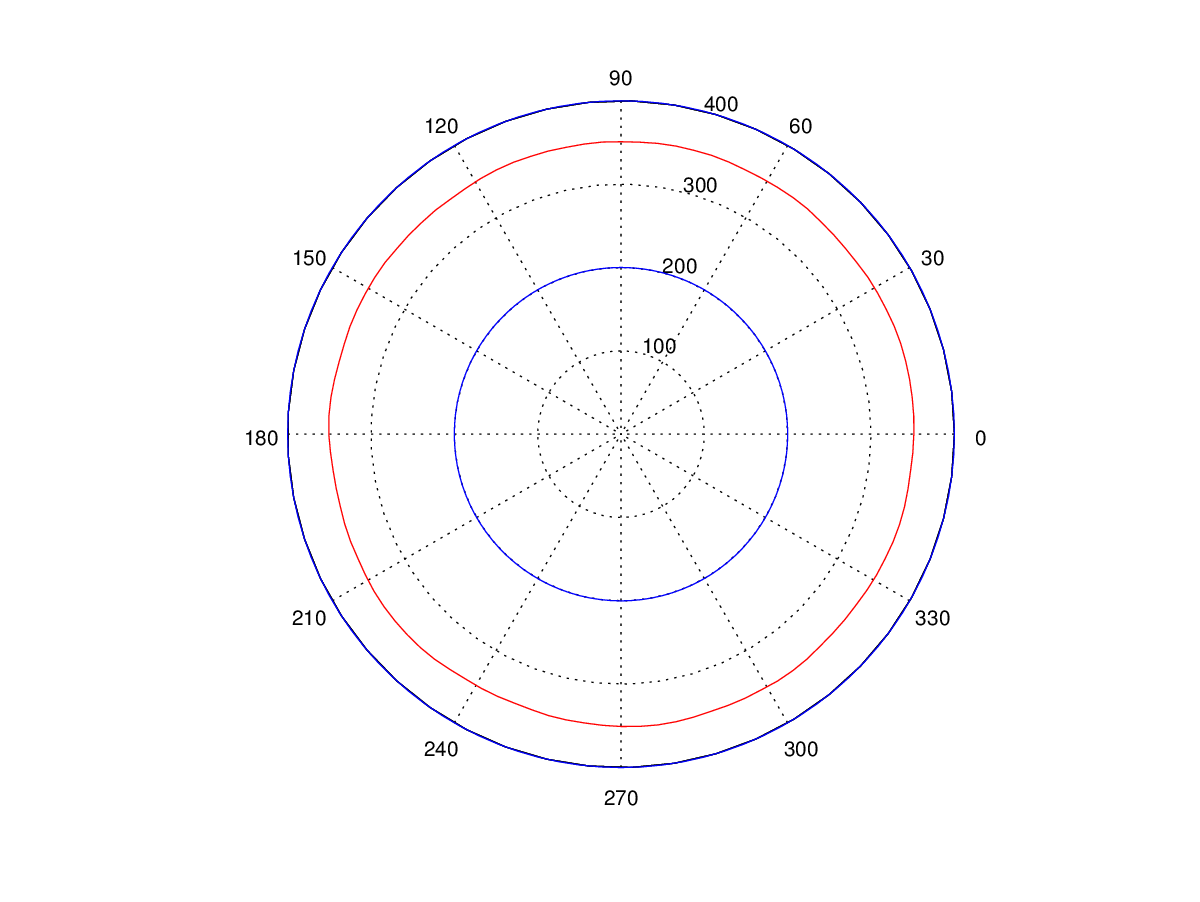
\includegraphics[scale=0.35]{experimentos1a_1b/evolucion_posicion_isoterma_temperatura/test2/test6_006_radios_inst_001_isomap.png}
	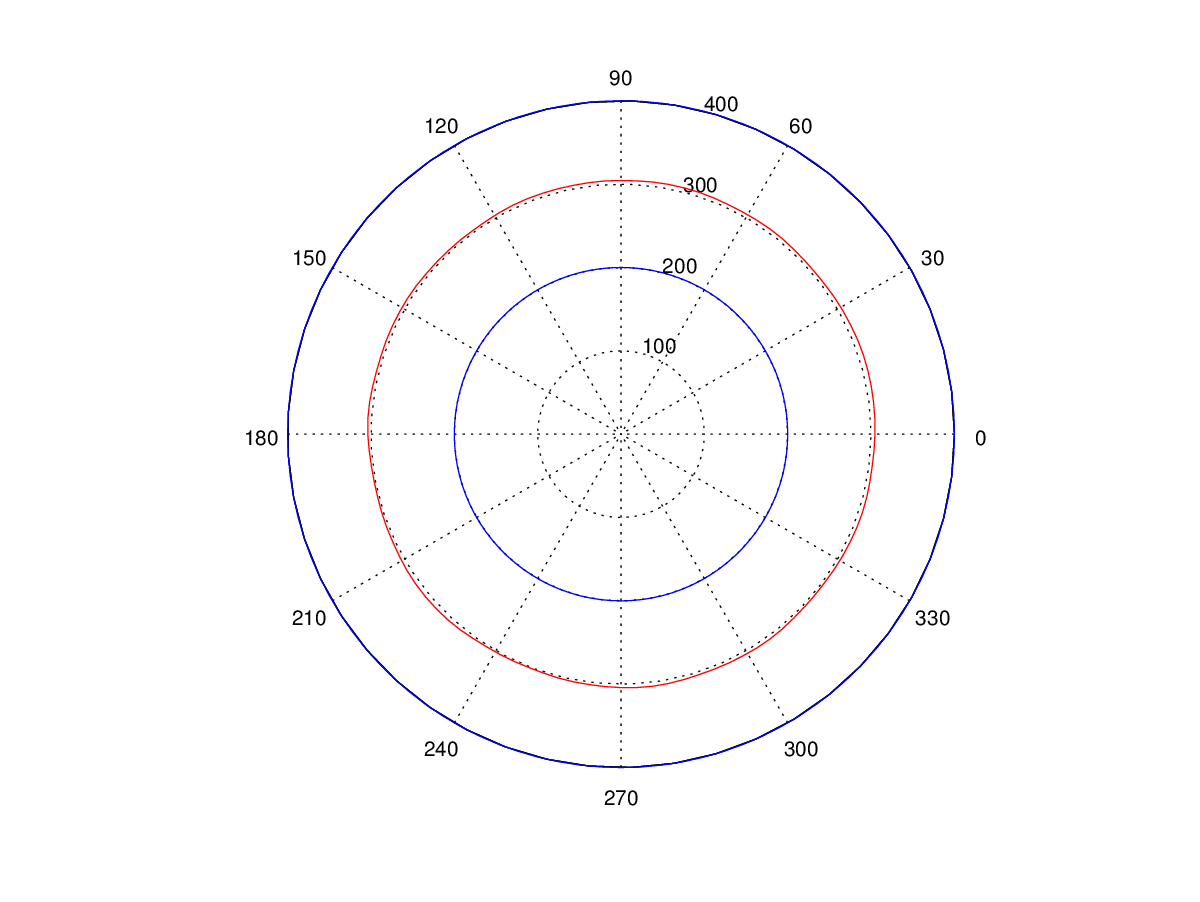
\includegraphics[scale=0.35]{experimentos1a_1b/evolucion_posicion_isoterma_temperatura/test2/test6_007_radios_inst_001_isomap.png}
	
  	\textbf{Variacion de la temperatura entre 6 y 7 radios de discretizacion}\\
	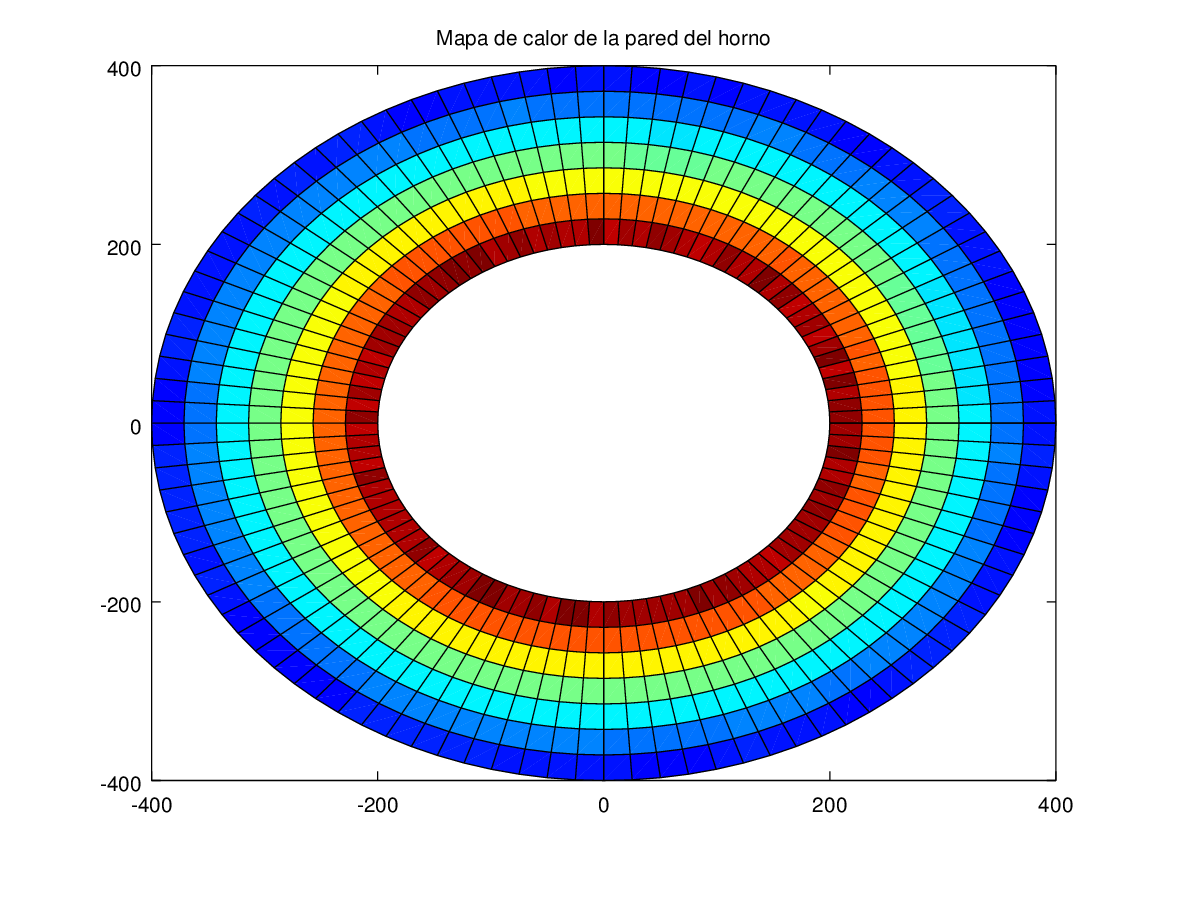
\includegraphics[scale=0.35]{experimentos1a_1b/evolucion_posicion_isoterma_temperatura/test2/test6_006_radios_inst_001_heatmap.png}
	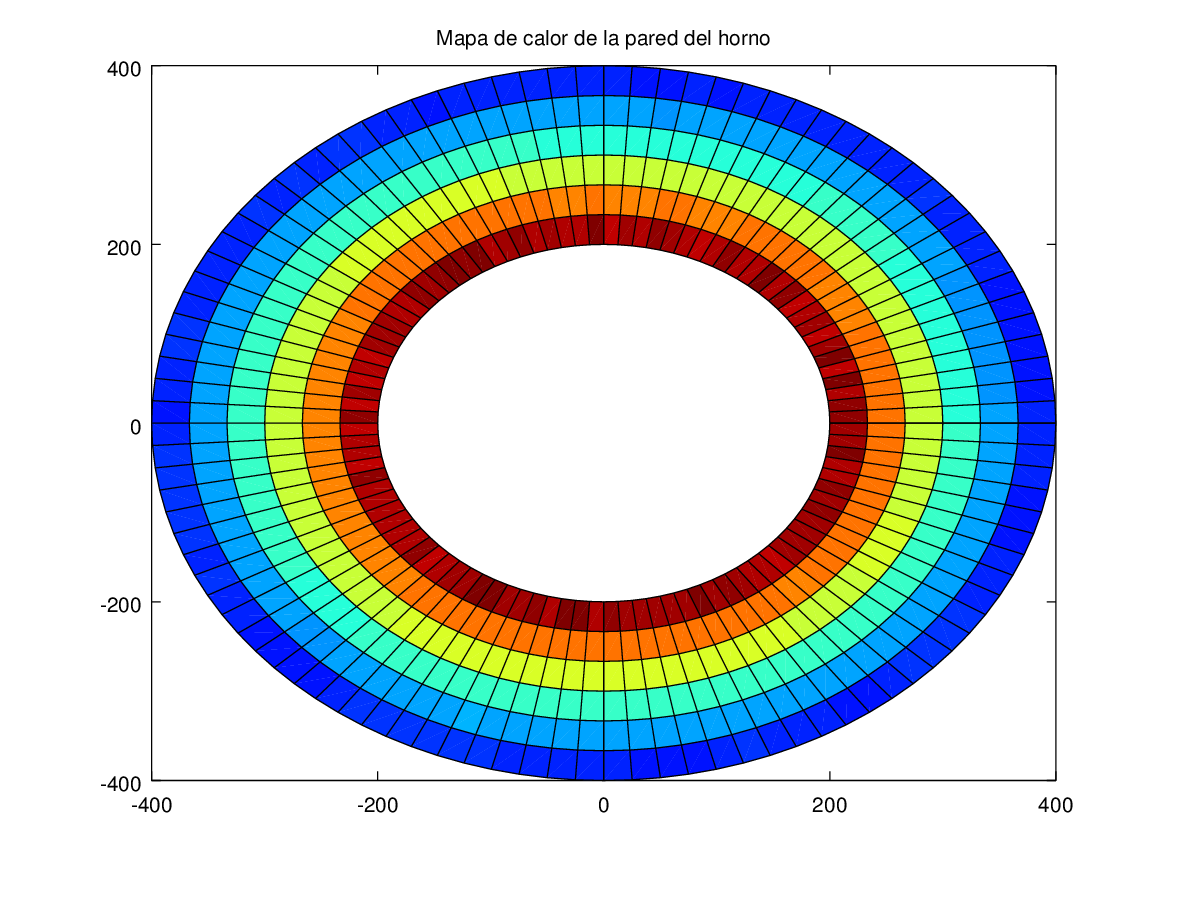
\includegraphics[scale=0.35]{experimentos1a_1b/evolucion_posicion_isoterma_temperatura/test2/test6_007_radios_inst_001_heatmap.png}

 	\textbf{Variacion de la estimacion de la isoterma entre 99 y 100 radios de discretizacion}\\
	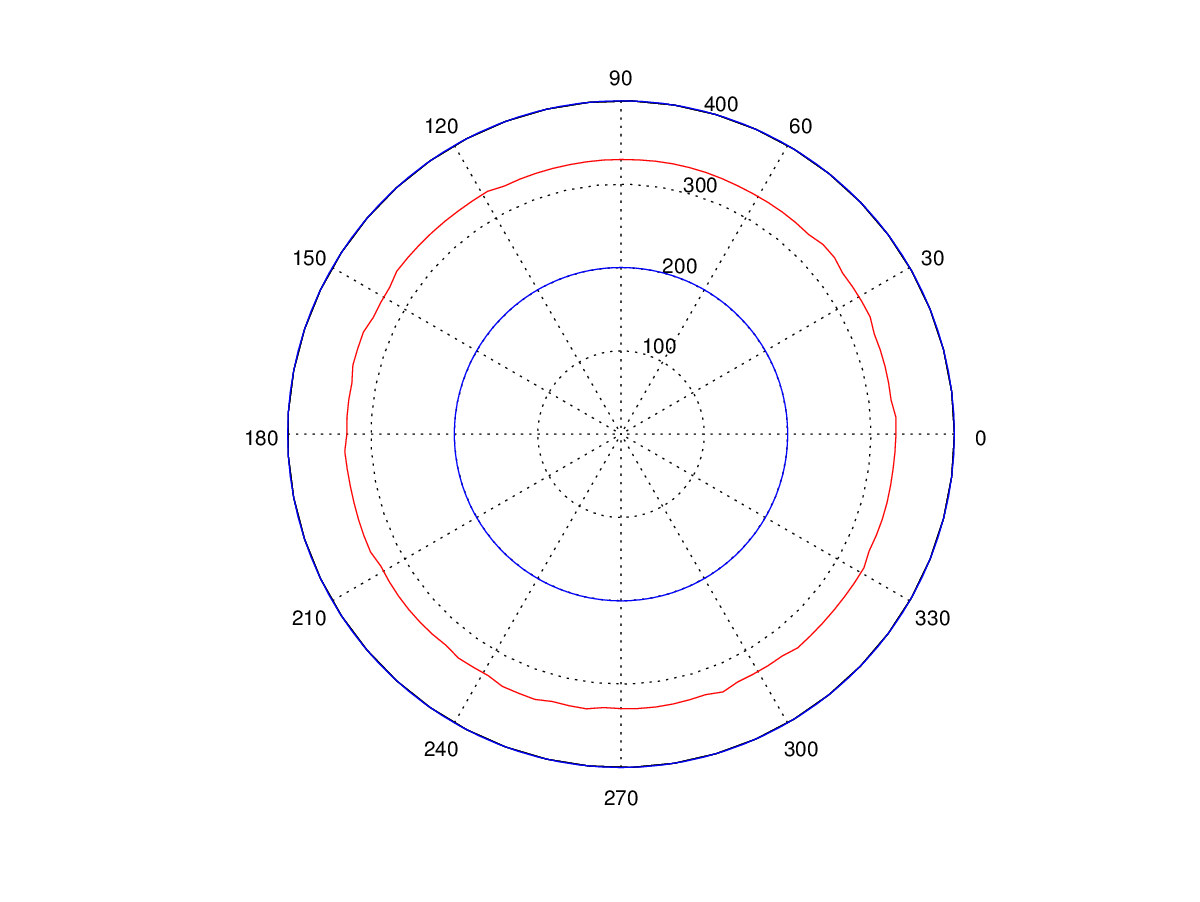
\includegraphics[scale=0.35]{experimentos1a_1b/evolucion_posicion_isoterma_temperatura/test2/test6_099_radios_inst_001_isomap.png}
	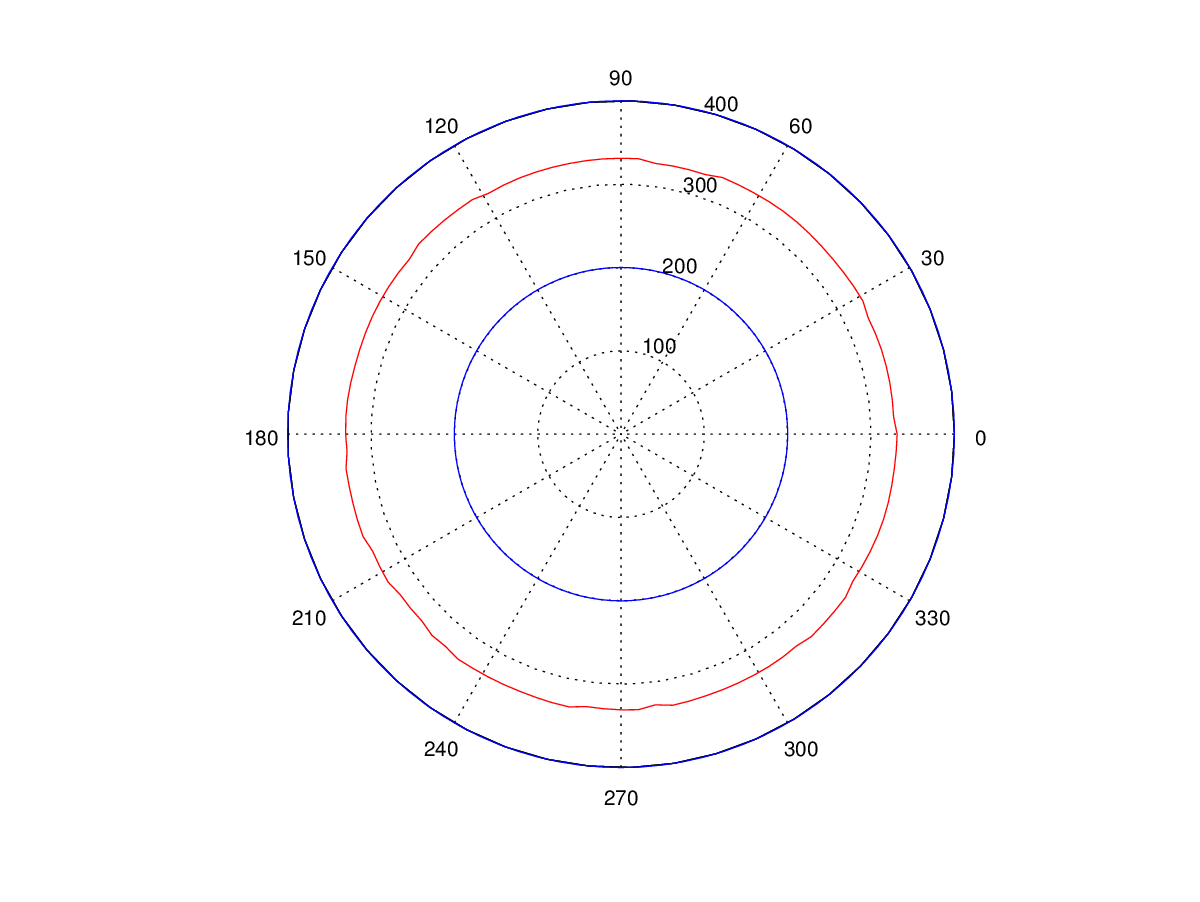
\includegraphics[scale=0.35]{experimentos1a_1b/evolucion_posicion_isoterma_temperatura/test2/test6_100_radios_inst_001_isomap.png}
	
	\textbf{Variacion de la temperatura entre 99 y 100 radios de discretizacion}\\
	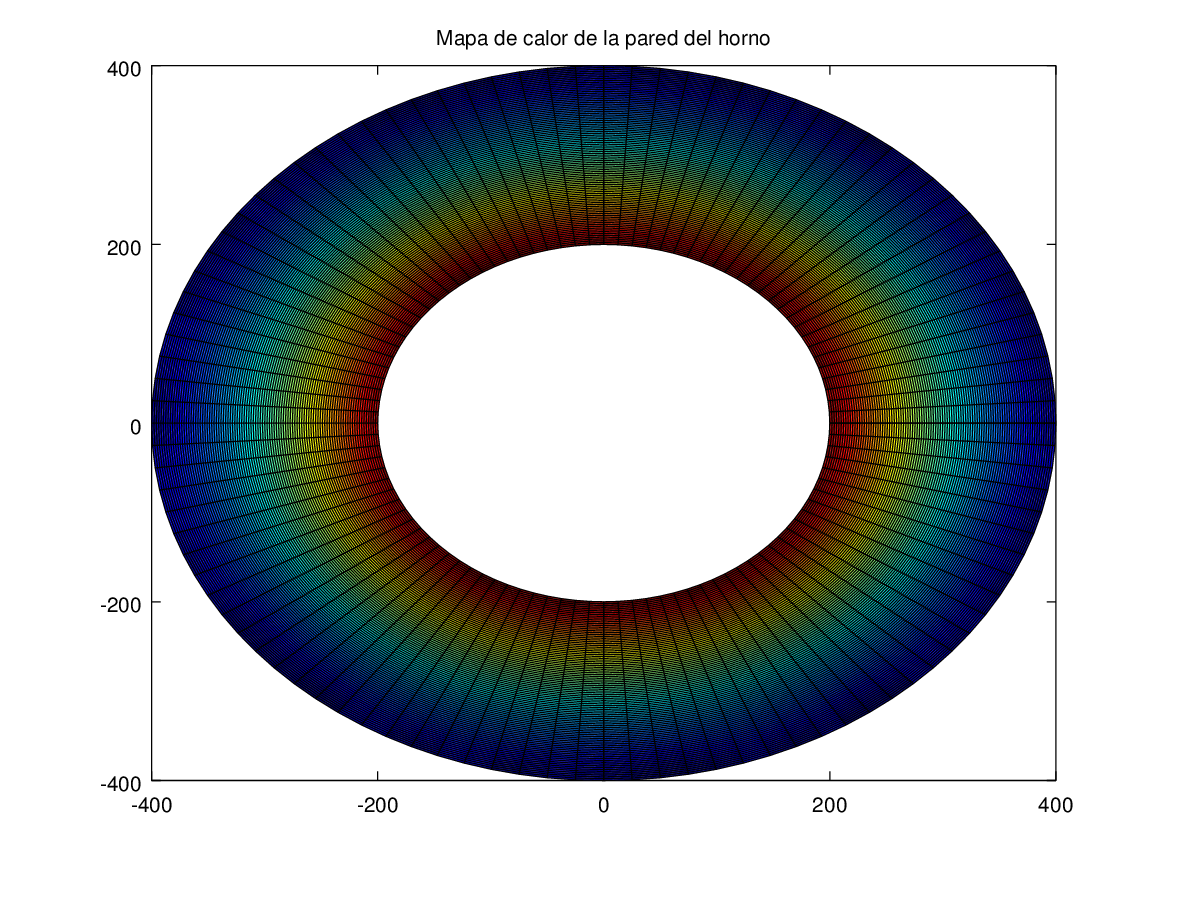
\includegraphics[scale=0.35]{experimentos1a_1b/evolucion_posicion_isoterma_temperatura/test2/test6_099_radios_inst_001_heatmap.png}
	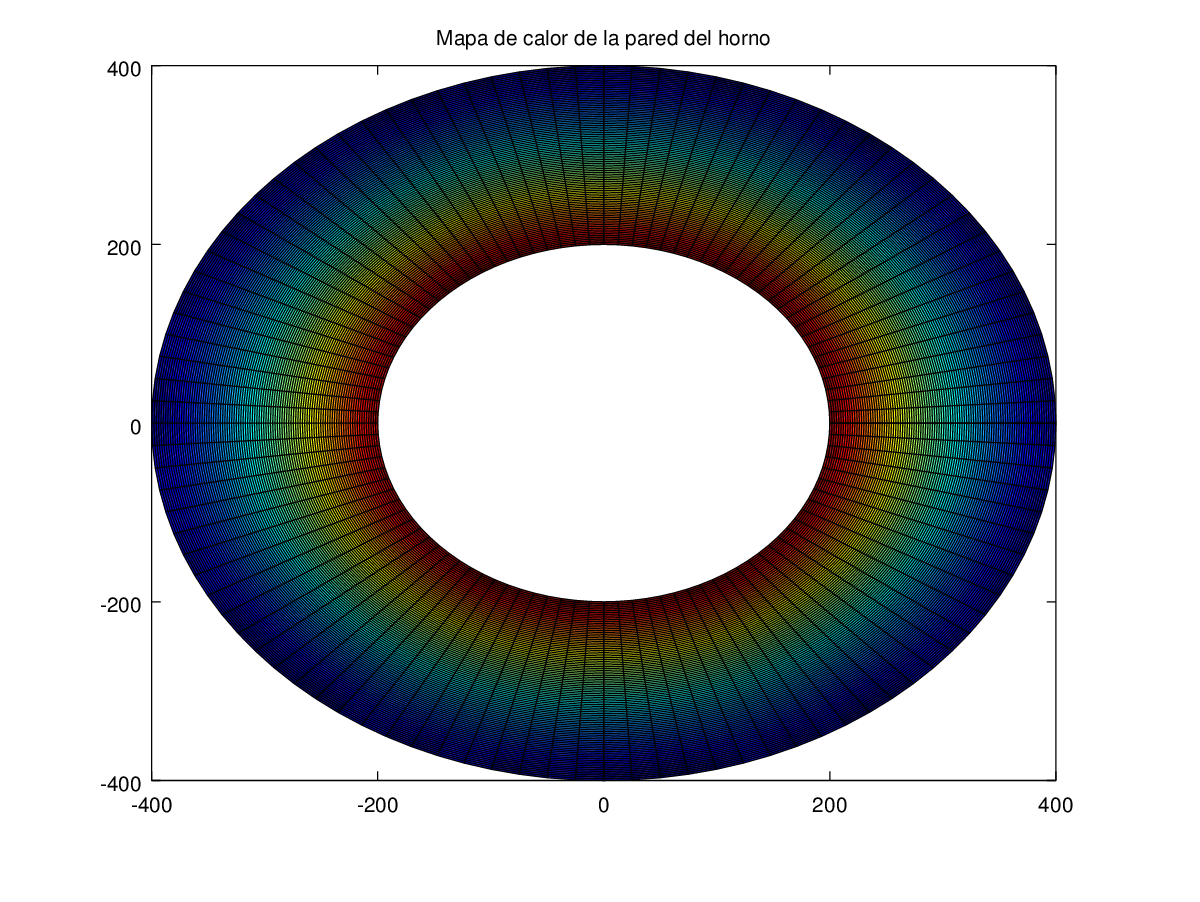
\includegraphics[scale=0.35]{experimentos1a_1b/evolucion_posicion_isoterma_temperatura/test2/test6_100_radios_inst_001_heatmap.png}

\vspace{0.5cm}

Se observa es que a medida que se aumenta la cantidad de radios de la discretizacion, la variacion radial de la curva de la isoterma disminuye entre tests, es decir, se hace mas fina la estimacion, de forma tal que entre $i$ e $i+1$ radios la diferencia de la posicion de la isoterma es menor a medida que $i$ crece. Para ver mejor esto se graficaron, para cada test de $i$ cantidad de radios de la discretizacion, el maximo y el promedio radial de la isoterma.

	\textbf{Evolucion de la variacion radial de la isoterma con cantidad creciente de radios}\\
	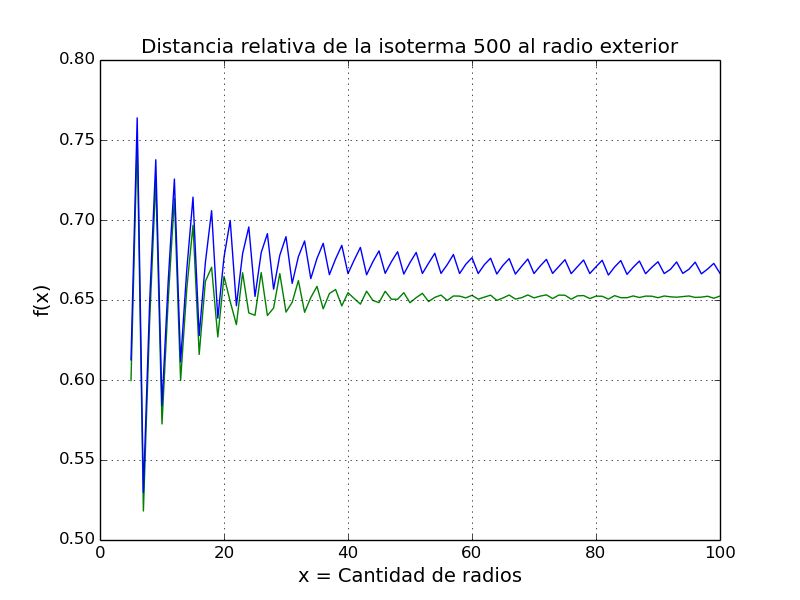
\includegraphics[scale=0.5]{experimentos1a_1b/evolucion_estimacion_seguridad_isoterma/100ang_5to100radios.png}\\

	\item \begin{itemize}
					\item \textbf{Temperaturas internas y externas:} constantes, 100 y 1500. Esto es para que tenga la misma solucion cada test del experimento.
					\item \textbf{Radio interno:} 200
					\item \textbf{Radio externo:} 400
					\item \textbf{Cantidad radios:} 50
					\item \textbf{Cantidad angulos:} $[5\dots50]$
					\item \textbf{Isoterma buscada:} 500
				\end{itemize}
	Se adjunta con el trabajo practico un video que expone la evolucion del sistema mientras se incrementa la cantidad de radios. Expondremos estaticamente algunos frames, pero es conveniente ver el video primero. Se encuentra en la misma carpeta que el pdf. (variacion\_angular\_isomap.mp4, variacion\_angular\_heatmap.mp4).

	\vspace{0.5cm}
	  	\textbf{Variacion de la estimacion de la isoterma entre 5 y 6 angulos de discretizacion}\\
		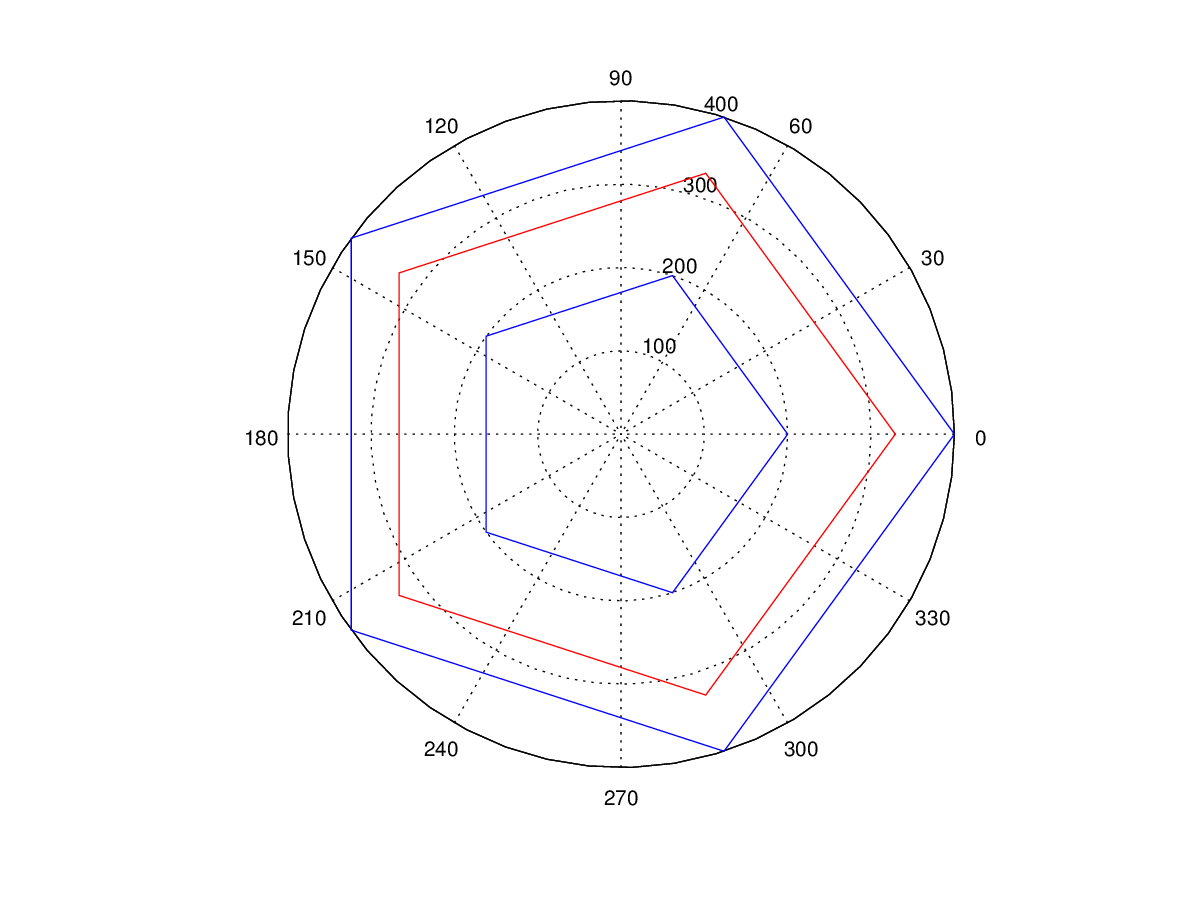
\includegraphics[scale=0.35]{experimentos1a_1b/evolucion_posicion_isoterma_temperatura/variacion_angulos_radio_fijo_se_suaviza_isoterma/test10_050_radios_005_angulos_inst_001_isomap.png}
		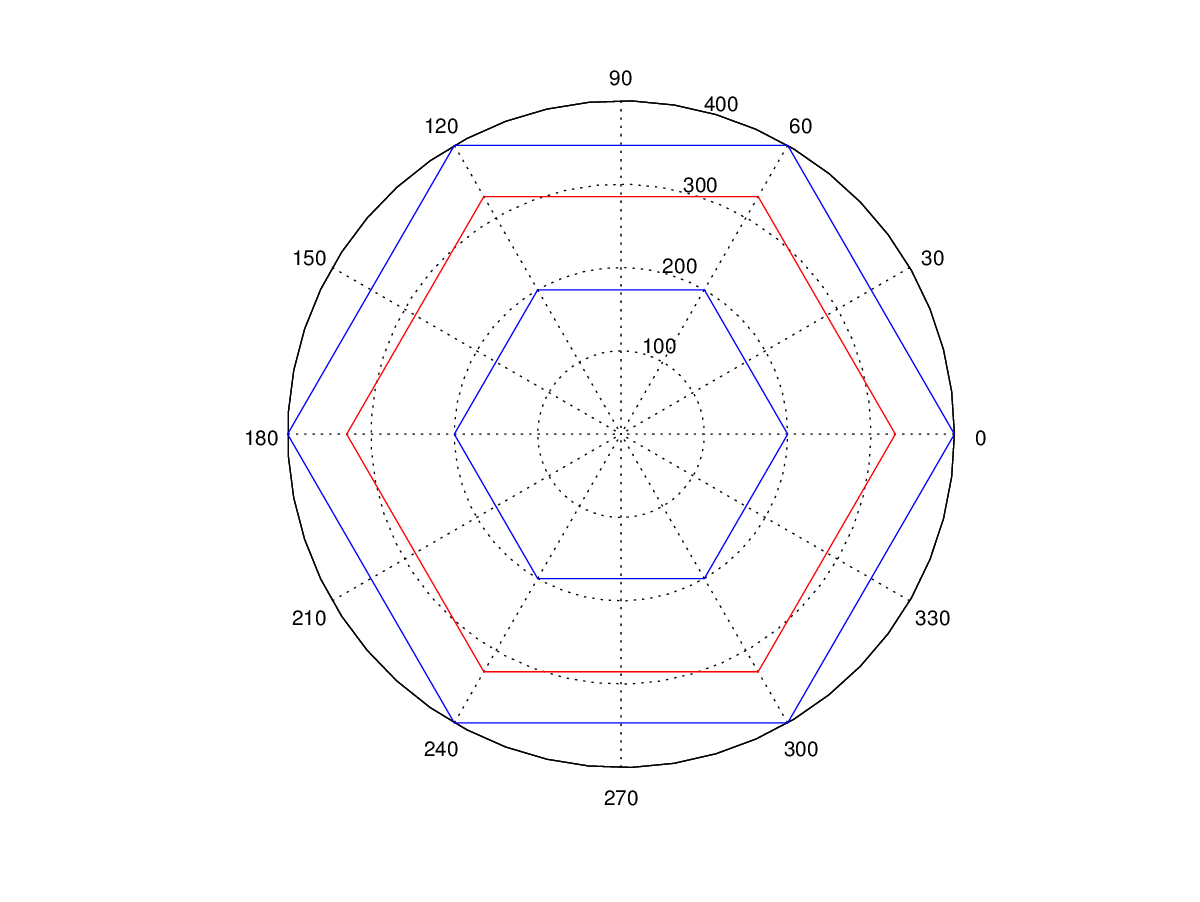
\includegraphics[scale=0.35]{experimentos1a_1b/evolucion_posicion_isoterma_temperatura/variacion_angulos_radio_fijo_se_suaviza_isoterma/test10_050_radios_006_angulos_inst_001_isomap.png}

	  	\textbf{Variacion de la temperatura entre 5 y 6 angulos de discretizacion}\\
	  	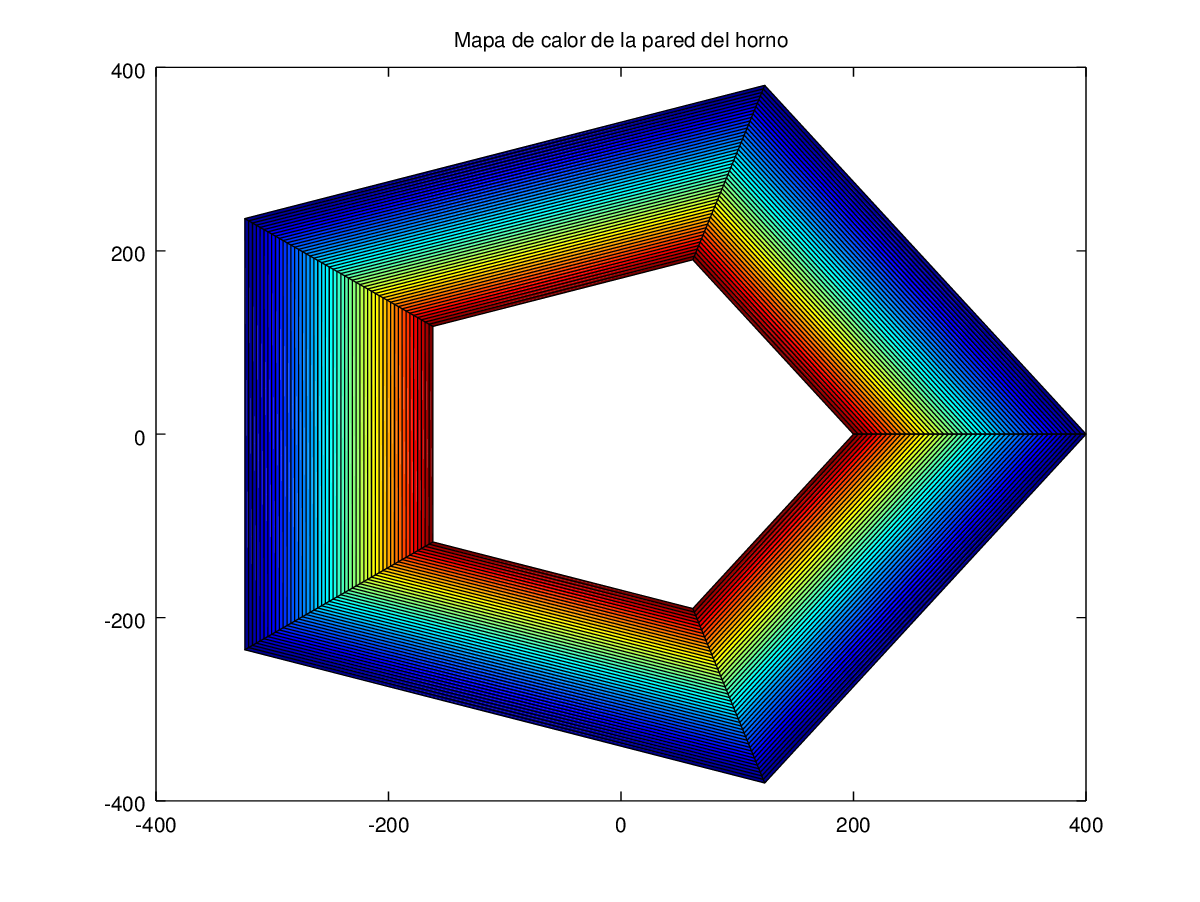
\includegraphics[scale=0.35]{experimentos1a_1b/evolucion_posicion_isoterma_temperatura/variacion_angulos_radio_fijo_se_suaviza_isoterma/test10_050_radios_005_angulos_inst_001_heatmap.png}
		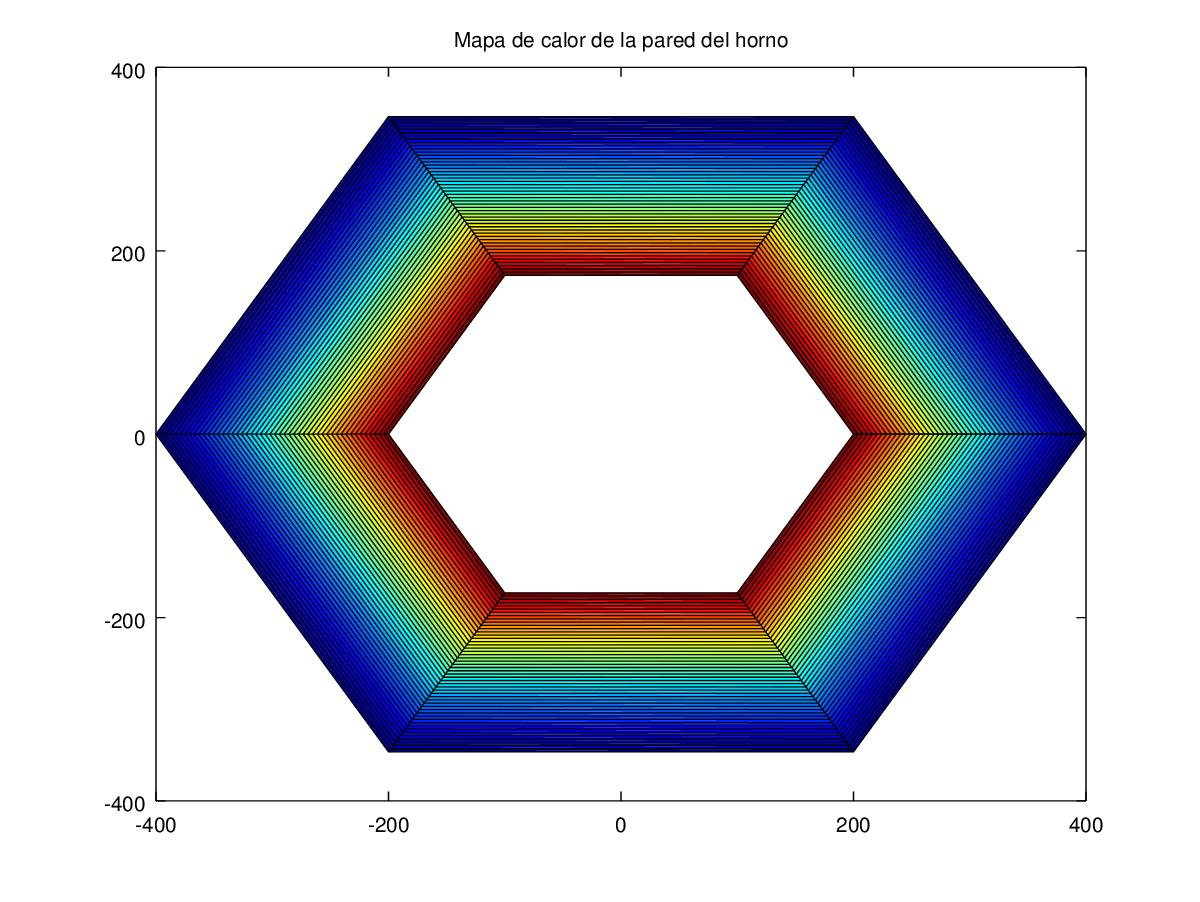
\includegraphics[scale=0.35]{experimentos1a_1b/evolucion_posicion_isoterma_temperatura/variacion_angulos_radio_fijo_se_suaviza_isoterma/test10_050_radios_006_angulos_inst_001_heatmap.png}	  	

	  	\textbf{Variacion de la estimacion de la isoterma entre 49 y 50 angulos de discretizacion}\\
		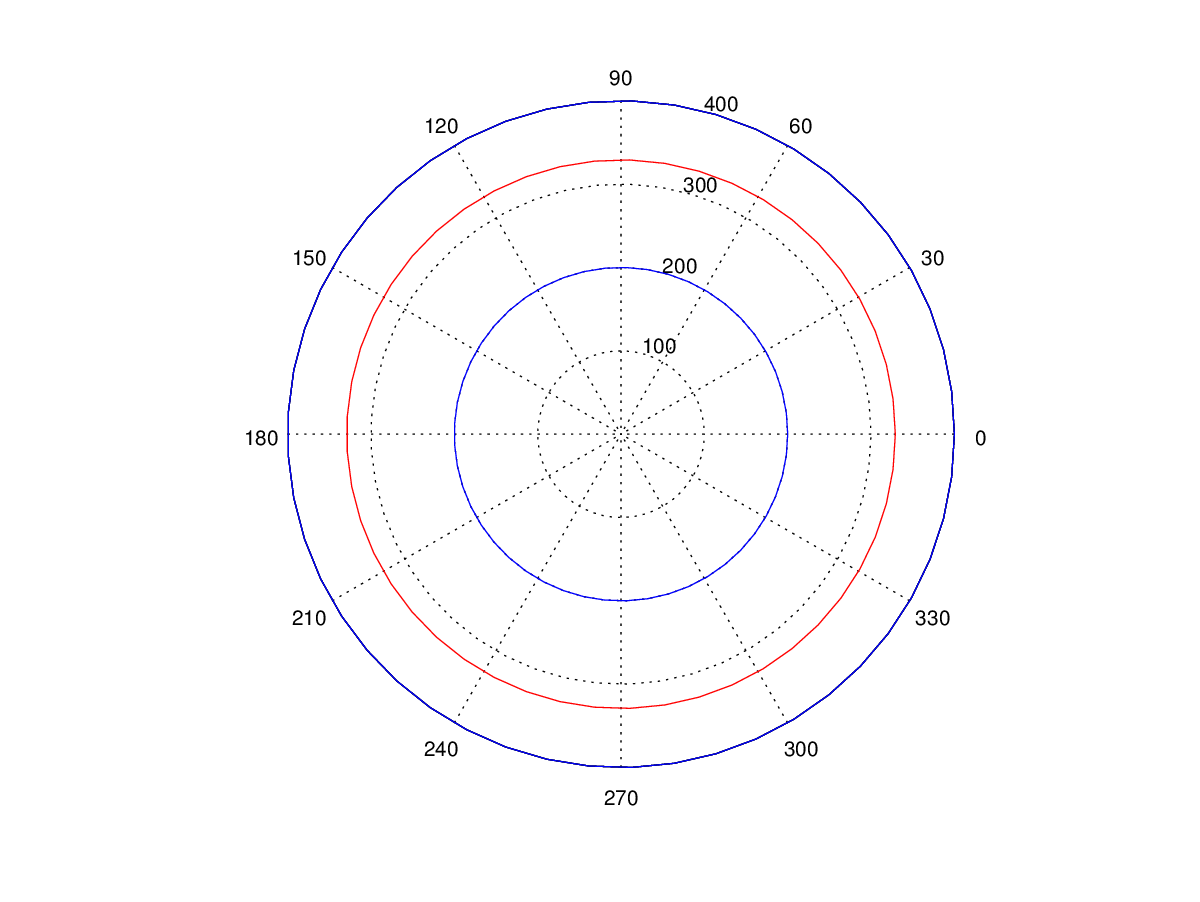
\includegraphics[scale=0.35]{experimentos1a_1b/evolucion_posicion_isoterma_temperatura/variacion_angulos_radio_fijo_se_suaviza_isoterma/test10_050_radios_049_angulos_inst_001_isomap.png}
		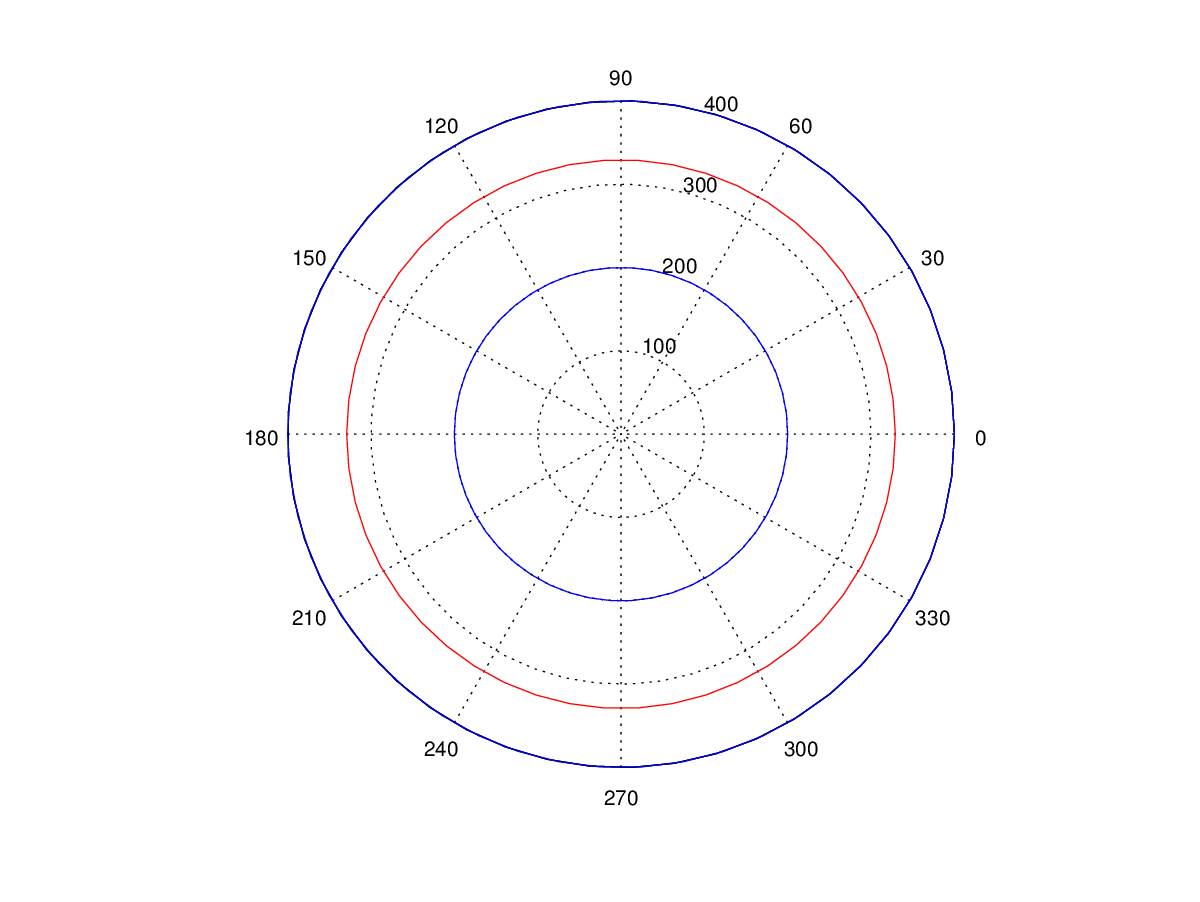
\includegraphics[scale=0.35]{experimentos1a_1b/evolucion_posicion_isoterma_temperatura/variacion_angulos_radio_fijo_se_suaviza_isoterma/test10_050_radios_050_angulos_inst_001_isomap.png}

		\textbf{Variacion de la temperatura entre 49 y 50 angulos de discretizacion}\\
	  	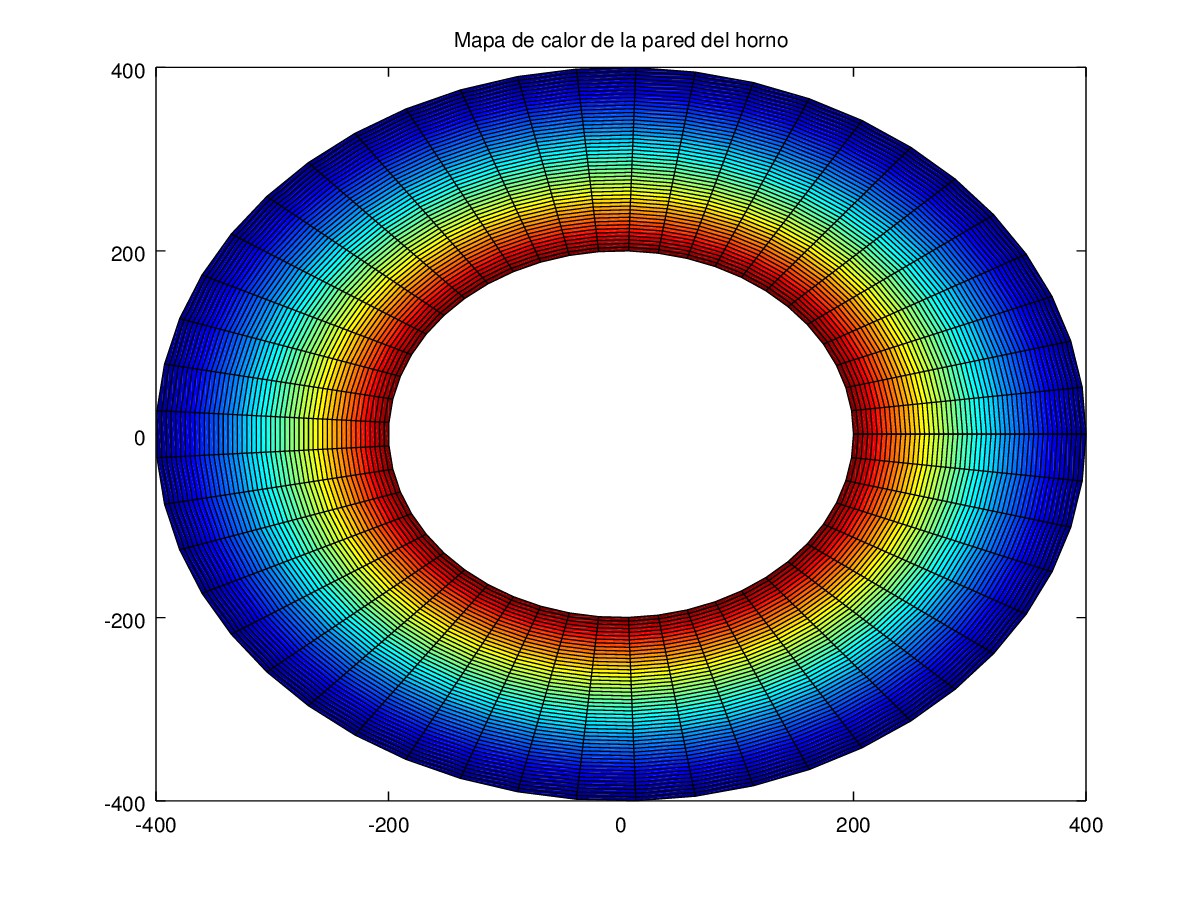
\includegraphics[scale=0.35]{experimentos1a_1b/evolucion_posicion_isoterma_temperatura/variacion_angulos_radio_fijo_se_suaviza_isoterma/test10_050_radios_049_angulos_inst_001_heatmap.png}
		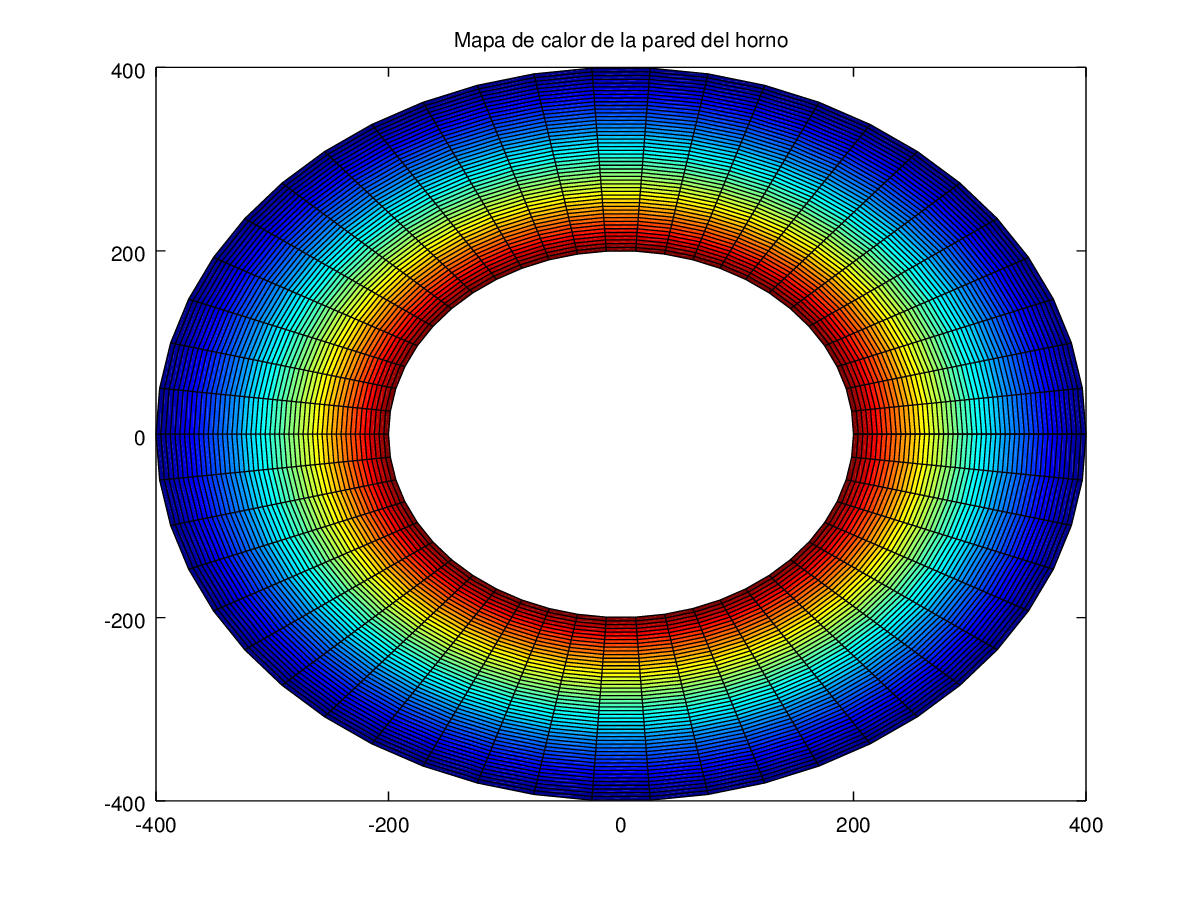
\includegraphics[scale=0.35]{experimentos1a_1b/evolucion_posicion_isoterma_temperatura/variacion_angulos_radio_fijo_se_suaviza_isoterma/test10_050_radios_050_angulos_inst_001_heatmap.png}

\vspace{0.5cm}

Aqui el radio es el mismo, pero se gana en precision al tener mas angulos por no tener que linealizar la posicion de la isoterma angularmente. Nuevamente, la posicion entre dos tests consecutivos se estabiliza al aumentar la cantidad de angulos. Tambien se observa que al cambiar el $\Delta_\theta$ los angulos entre tests consecutivos no son los mismos.

	\item \begin{itemize}
						\item \textbf{Temperaturas internas y externas:} constantes, 100 y 1500. Esto es para que tenga la misma solucion cada test del experimento.
						\item \textbf{Radio interno:} 200
						\item \textbf{Radio externo:} 400
						\item \textbf{Cantidad radios:} $[15\dots60]$
						\item \textbf{Cantidad angulos:} $[15\dots60]$
						\item \textbf{Isoterma buscada:} 500
					\end{itemize}
	Se adjunta con el trabajo practico un video que expone la evolucion del sistema mientras se incrementa la cantidad de radios. Expondremos estaticamente algunos frames, pero es conveniente ver el video primero. Se encuentra en la misma carpeta que el pdf. (variacion\_doble\_isomap.mp4, variacion\_doble\_heatmap.mp4).

	\vspace{0.5cm}
	  	\textbf{Variacion de la estimacion de la isoterma entre 15 y 16 radios, angulos de discretizacion}\\
		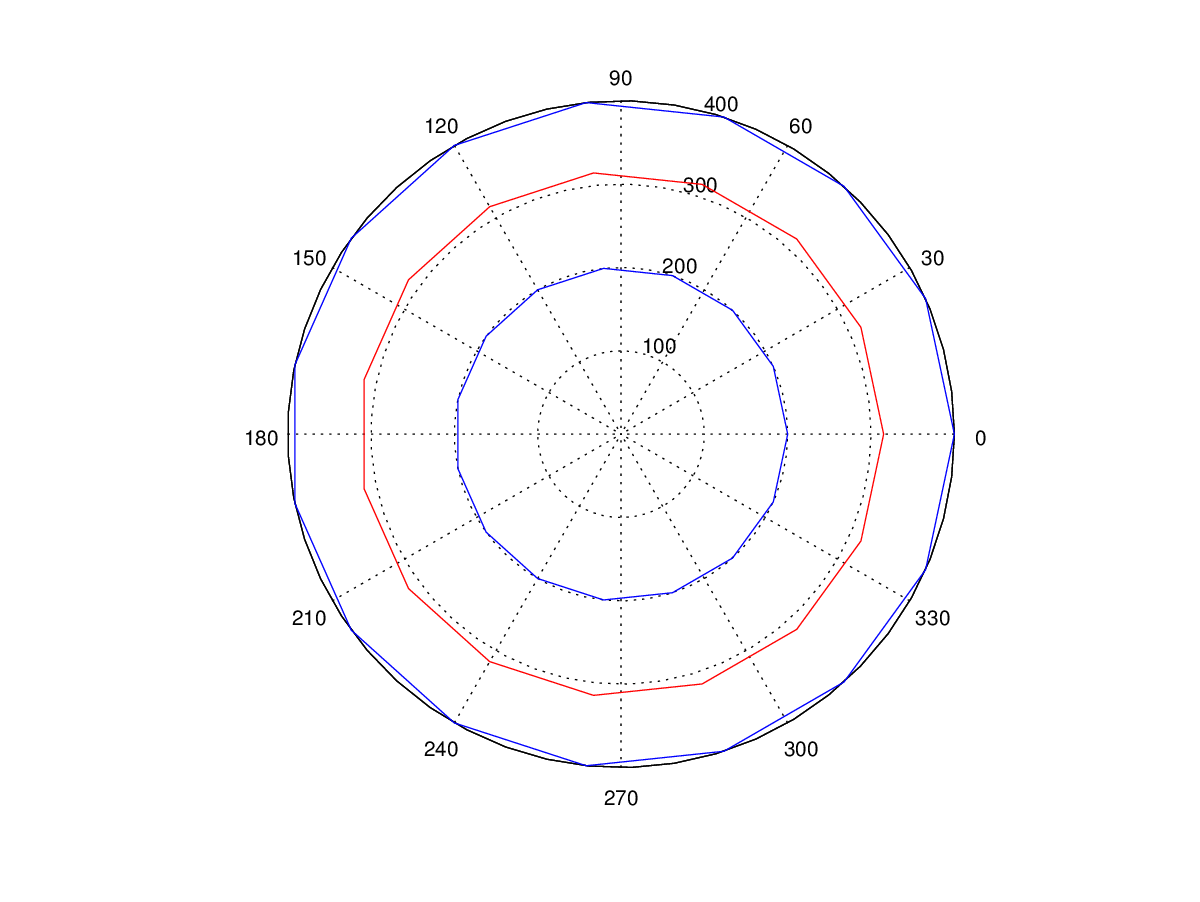
\includegraphics[scale=0.35]{experimentos1a_1b/evolucion_posicion_isoterma_temperatura/variacion_radios_angulos_se_reduce_diferencia_radial/test11_testord_001_inst_001_isomap.png}
		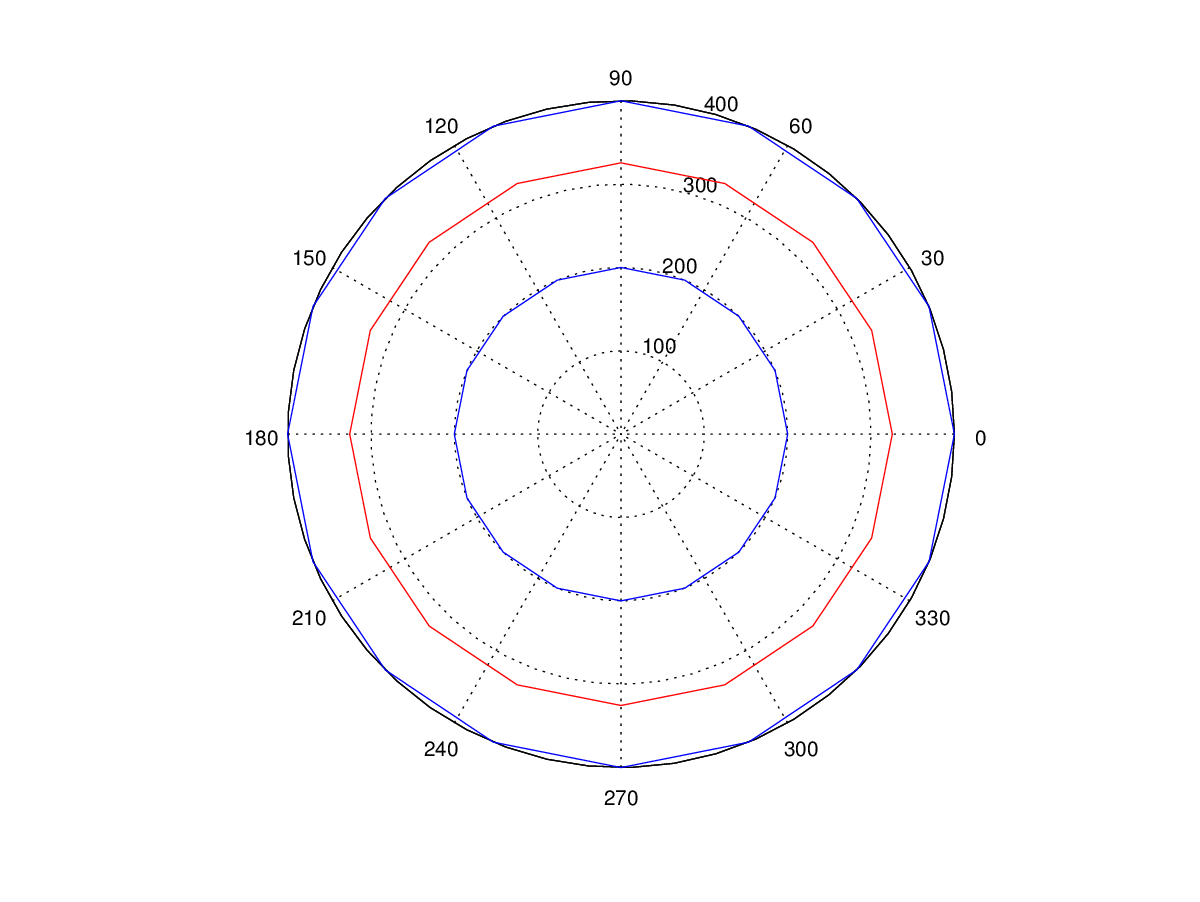
\includegraphics[scale=0.35]{experimentos1a_1b/evolucion_posicion_isoterma_temperatura/variacion_radios_angulos_se_reduce_diferencia_radial/test11_testord_002_inst_001_isomap.png}

	  	\textbf{Variacion de la temperatura entre 59 y 60 radios, angulos de discretizacion}\\
	  	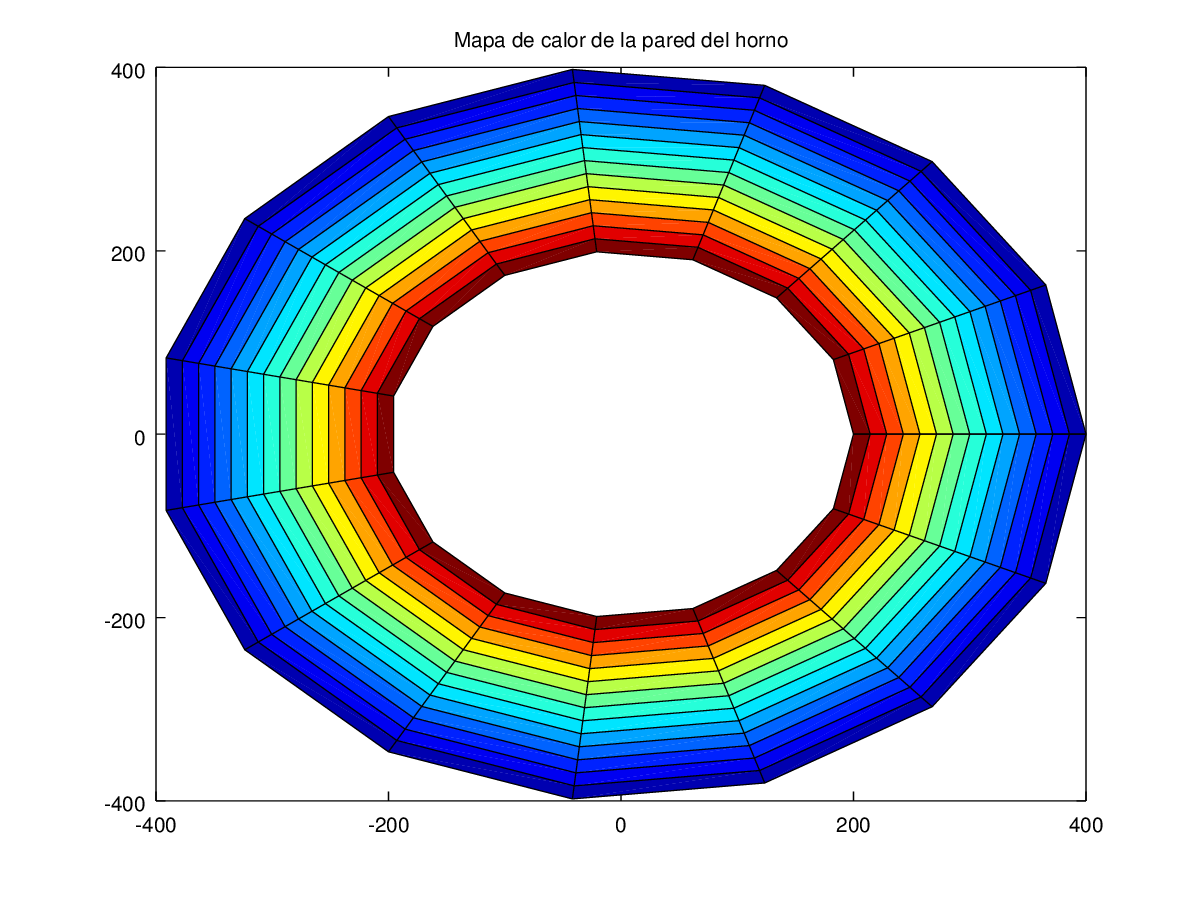
\includegraphics[scale=0.35]{experimentos1a_1b/evolucion_posicion_isoterma_temperatura/variacion_radios_angulos_se_reduce_diferencia_radial/test11_testord_001_inst_001_heatmap.png}
		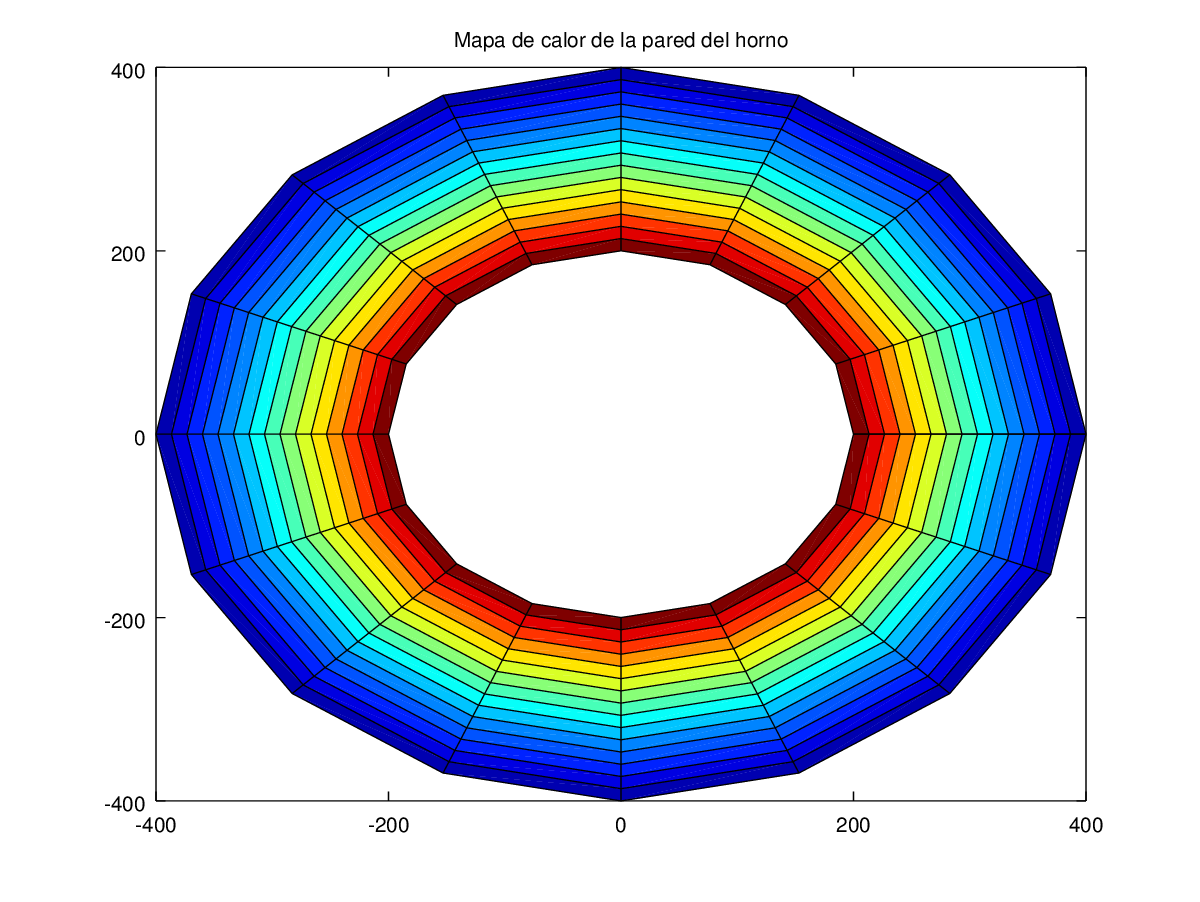
\includegraphics[scale=0.35]{experimentos1a_1b/evolucion_posicion_isoterma_temperatura/variacion_radios_angulos_se_reduce_diferencia_radial/test11_testord_002_inst_001_heatmap.png}

	  	\textbf{Variacion de la estimacion de la isoterma entre 15 y 16 radios, angulos de discretizacion}\\
		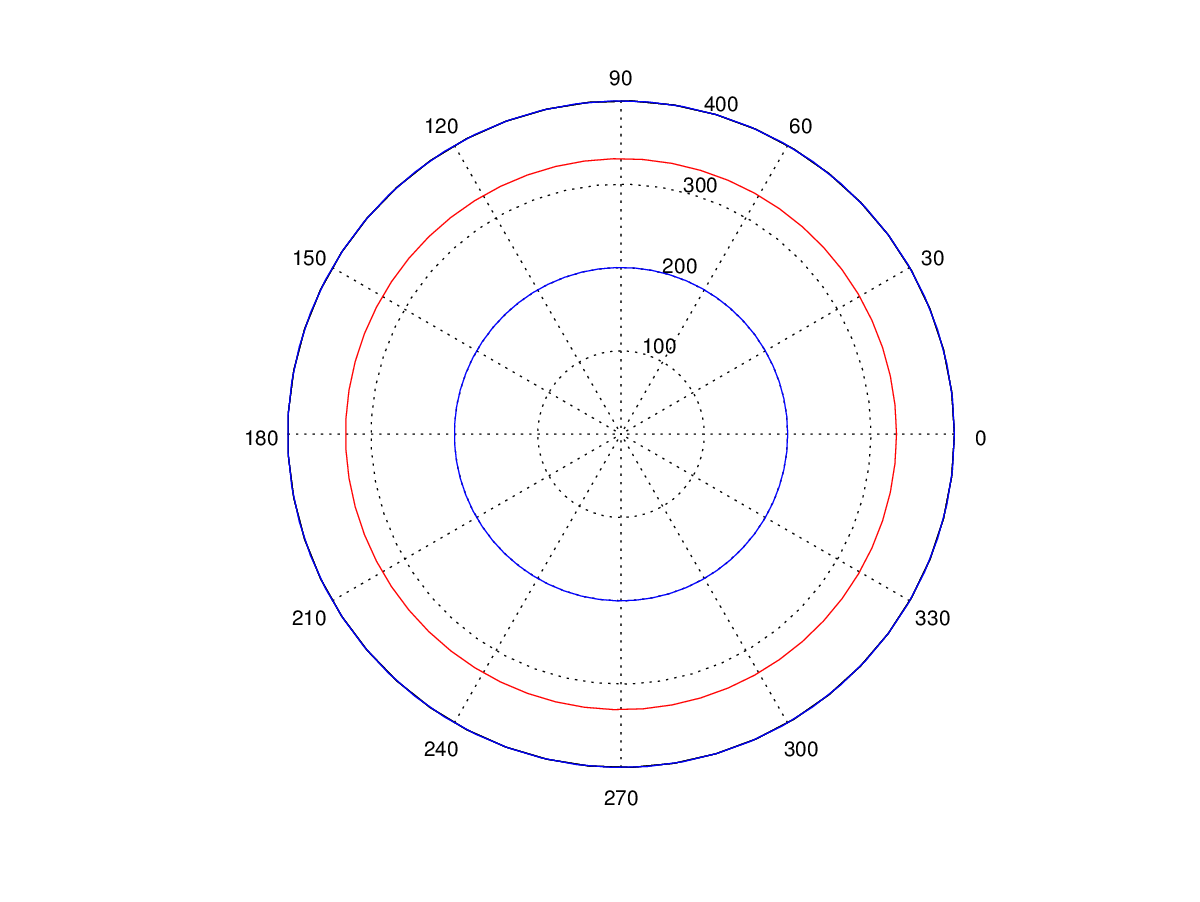
\includegraphics[scale=0.35]{experimentos1a_1b/evolucion_posicion_isoterma_temperatura/variacion_radios_angulos_se_reduce_diferencia_radial/test11_testord_045_inst_001_isomap.png}
		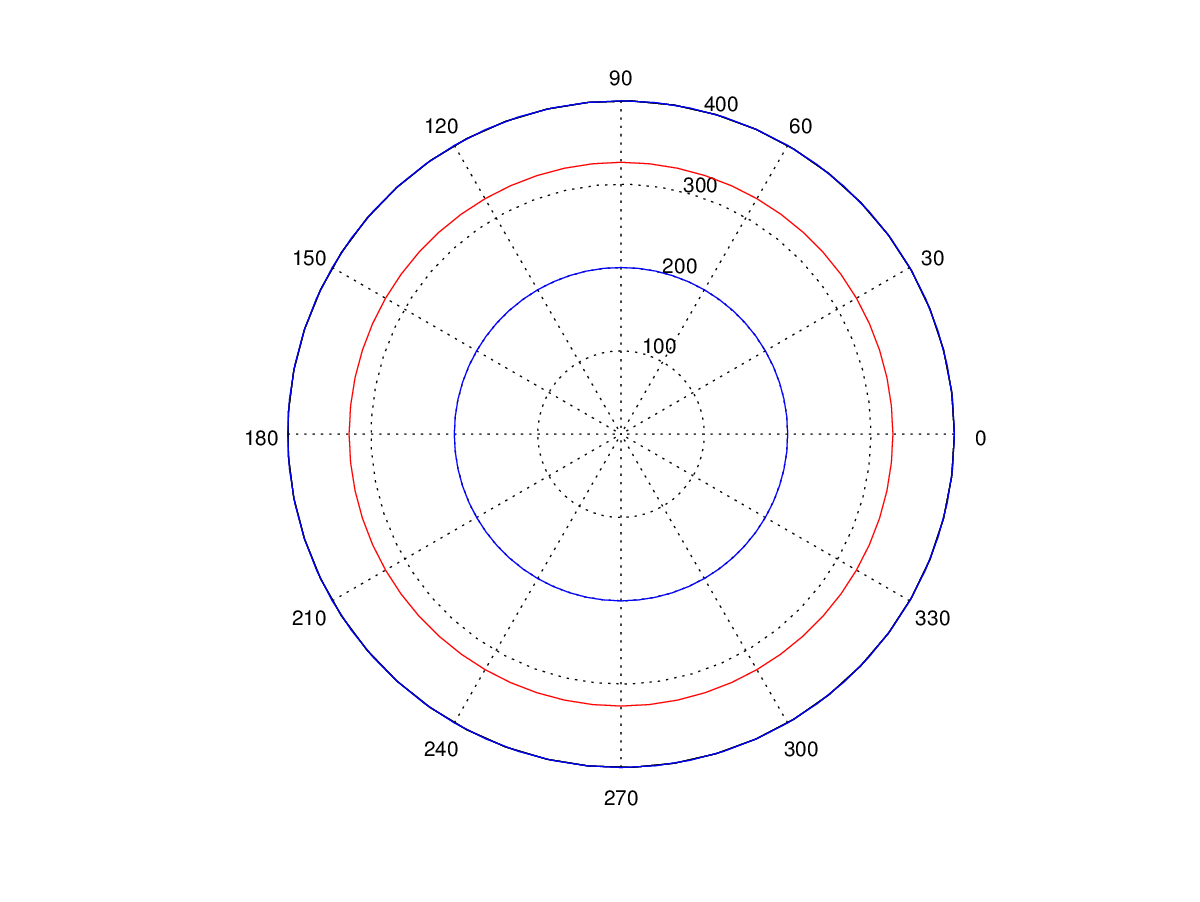
\includegraphics[scale=0.35]{experimentos1a_1b/evolucion_posicion_isoterma_temperatura/variacion_radios_angulos_se_reduce_diferencia_radial/test11_testord_046_inst_001_isomap.png}

		\textbf{Variacion de la temperatura entre 59 y 60 radios, angulos de discretizacion}\\
	  	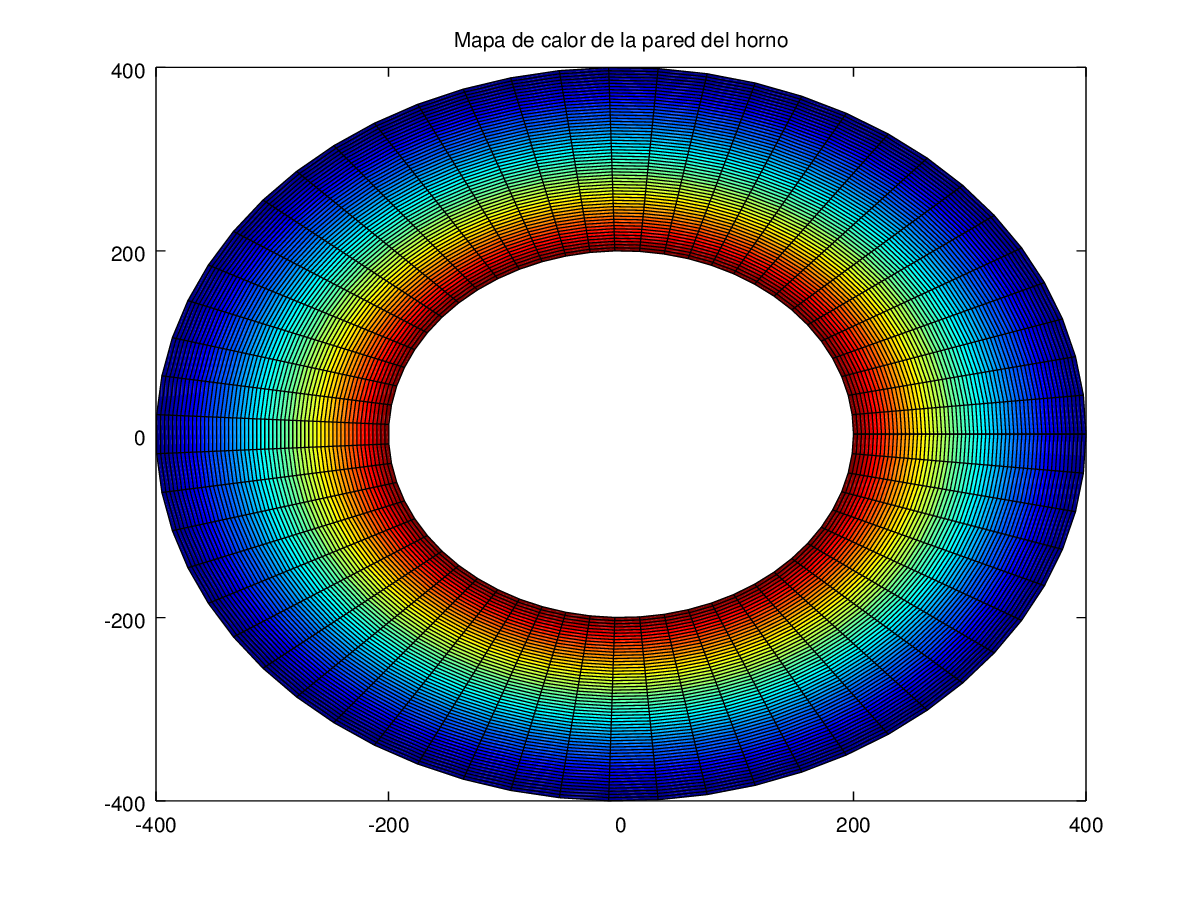
\includegraphics[scale=0.35]{experimentos1a_1b/evolucion_posicion_isoterma_temperatura/variacion_radios_angulos_se_reduce_diferencia_radial/test11_testord_045_inst_001_heatmap.png}
		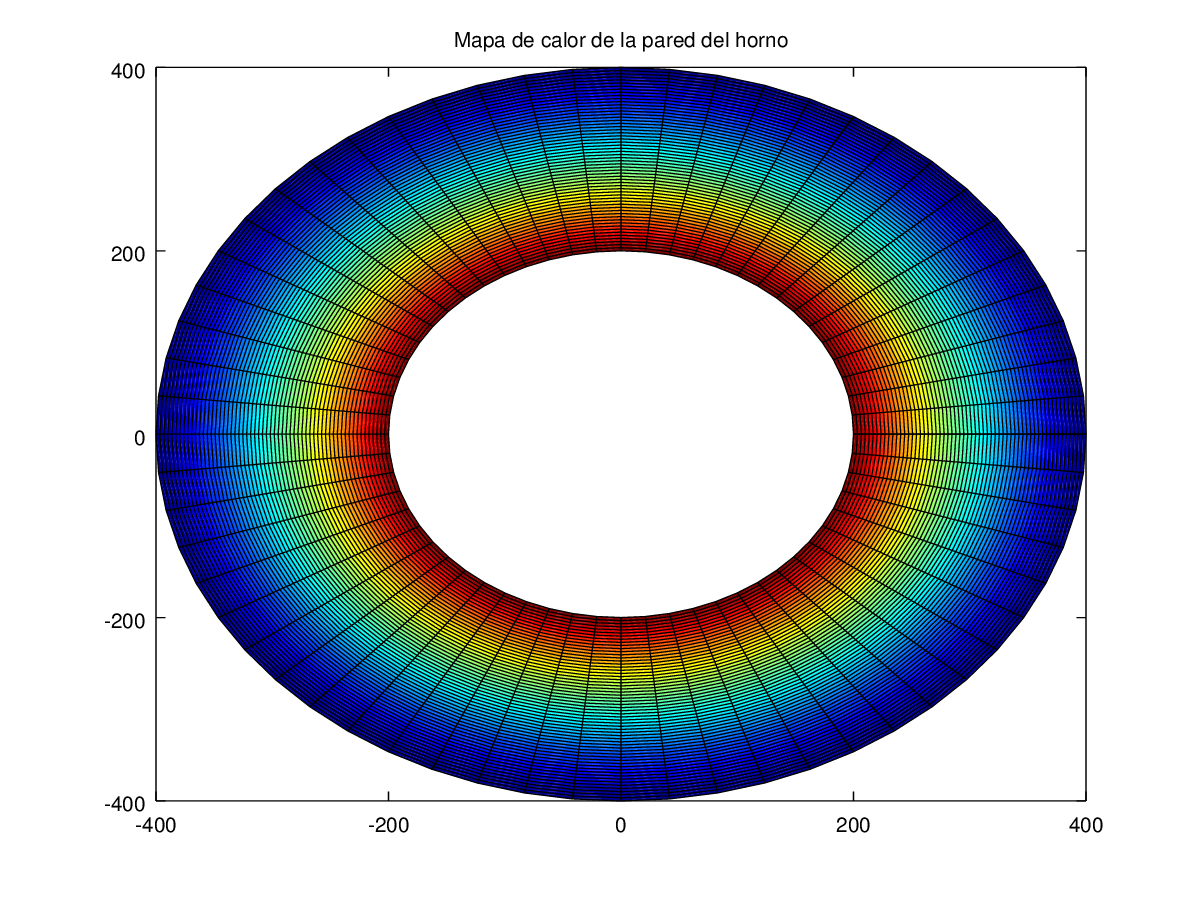
\includegraphics[scale=0.35]{experimentos1a_1b/evolucion_posicion_isoterma_temperatura/variacion_radios_angulos_se_reduce_diferencia_radial/test11_testord_046_inst_001_heatmap.png}

\vspace{0.5cm}

En este ultimo ejemplo ocurren ambos fenomenos al mismo tiempo, hay una variacion radial menor a medida que crecen los radios y la curva se suaviza al aumentar los angulos.

\end{enumerate}

\vspace{0.5cm}

Efectivamente, podemos concluir que mientras mas fina sea la discretizacion, se obtendran resultados mas \texttt{estables y confiables} acerca de la estimacion. Uno de los motivos es porque habrá menos puntos para interpolar en la posicion de la isoterma y el otro porque se tiene mas informacion de la temperatura de la pared del horno.

\subsubsection{Estimacion de estabilidad de la pared del horno}
poner imagenes bien elegidas entre las que hiciste. aclarar que el color del heatmap es relativo al minimo y maximo de la muestra, por eso temperaturas altas afuera sigue siendo azul.